\documentclass[]{article}

\usepackage{graphicx} % dla obrazków
\graphicspath{ {./images/} }

\usepackage{amsmath}
\usepackage{algorithm}
\usepackage[noend]{algpseudocode} %pseudocode

%opening
\title{}
\author{Karolina Drabent \\ Patryk Fijałkowski \\ Artur Haczek \\ Krzysztof Kamiński \\ Pamela Krzypkowska}



\begin{document}

\maketitle

\begin{abstract}
	
\par This short paper will cover the topic of Q-Learning tested on an Agent base input game, which in our scenario is a simple Snake game. We will first explain what Q-Learning is, how and why it works and what is it used for. Later we will present our solution with the usage of Q-Learning methods which goal is to teach an Agent to play our Snake game, maximise its score and amount of moves per game. Finally we would show how our method is working in practise, what changes could be made further on as well as different approaches that we had encountering numerous problems along with their actual outcomes.

\end{abstract}

\section{Background Knowledge}

\subsection{Q Learning}

\par Q Learning is one of the Reinforcement Learning paradigm methods. This is a method somewhere close to unsupervised learning, which is a Machine Learning method which centres around learning without a teacher. A teacher is usually represented by a data-set or a set of labels and observed outcomes. Q Learning is based on a reward given to an agent after an action the agent has performed in a given environment. The environment is always a model providing positive or negative rewards to agent. 

\par The goal of this learning method is to teach an agent, which decisions to make under which circumstances. Therefore the agent's goal is to create its own model of the environment, not known to the agent at all before the active learning process starts. The agent is changing its future decisions based on the rewards from its actions - building the model previously mentioned. 

\par The classic Q Learning is based on a Q table which is a reward function presented as a matrix. This function returns the value of a Q function having the previous action chosen being A and previous state (before performing a given action A) being Q (The function will be explained later, the main focus is that the system counts the values in Q table based on previous state, action chosen and reward given from the environment). Firstly the Q table is filled with a neutral element (it can also be any arbitrary value chosen by a programmer), when we are using real numbers the neutral element would be 0. Therefore the Q table has a following function signature: 
\begin{equation}
Q : S \times A \rightarrow \rm I\!R
\end{equation}

\par The process of updating values in the Q table which tells us what reward can be given to an agent being in state Q, performing action action A is made based on iterations. Before deciding the next actions, agent checks the Q-table and learns which action would be the most profitable based on its previous knowledge of rewards provided. Every iterations gives the system more information because after every action it updates the Q table with the new value of reward-based-value given on action A performed from state Q. The value put inside the Q table is obtained with the following equation \ref{fig:qlearn}, presented below: 

\begin{figure}[h]
	\centering
	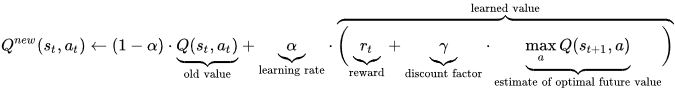
\includegraphics[scale=0.6]{qlearn}
	\caption{Q function}
	\label{fig:qlearn}
\end{figure}

\par The values such as the learning rate and discount factor are there to be tweaked by human agents building the model. Learning rate being a level to which new information overrides old information (how much the Q table is going to be changed after new information is gained) and discount factor is a way of making agent more far-sighted, so it would also value long term rewards that might be gained, not only short term rewards which might be smaller. 

\par The system finished the learning when it reaches the final state. After the final state, the model (meaning the Q table) can be used for next iterations to enable to agent to teach itself better while working with the environment, updating its knowledge with every iteration. It's important to note that there might be no final state, and the Q Learning algorithm can also be used in such situations. 

\subsection{Deep Q Learning}

\par The method we have chosen in our project is a Deep Q Learning, which is a method of Q Learning using Deep neural networks. In Deep Q Learning there is no Q table, which is a model of environment created by the agent. The model of the environment is contained in the network. This network can be called a Q Network, this network outputs the predicted reward for the agent, given actions it can perform.

\subsection{Agent input games}

\par Snake is a very simple game, which originated back in the XXth Century. It is quite popular to use simple games in which a human agent inputs sequences, to showcase popular Machine Learning algorithms, especially neural networks. In this examples a input usually generated by a human is changed so that the input is generated by a computer program (we can also call it an agent). 

\par Having games with points to collect or score like Pacman, Space Impact or Snake it is an interesting case study to implement reinforcement learning methods, trying to make the agent learn to play the game from externally provided rewards. Rewards correlate with point that the player is collecting and the time for which it can stay alive. Many of those games not only enable the player to score points, but also have some actions lead to a death of a player and loosing all points. A learning agent is then facing a problem of optimizing the risks along with potential gains. 

\par It is quite important to note that this is a simplified model of a very low-level human-like learning process based on rewards.

\section{Our methods}

\subsection{Environment}

\par As mentioned before we are training an agent to learn how to play snake. I won't get into details of architecture of the game itself, because it is not too important. The crucial part lies in a model of the environment and what we want to teach our agent. We want to teach our snake to learn how to score as many points as possible and live as long as possible. Points are scored when the agent is moving on a board of fixed size, and is eating apples. The maximum number of points available for the player is bounded by the board size. The game UI is showed on the picture \ref{fig:snake} below:

\begin{figure}[h]
	\centering
	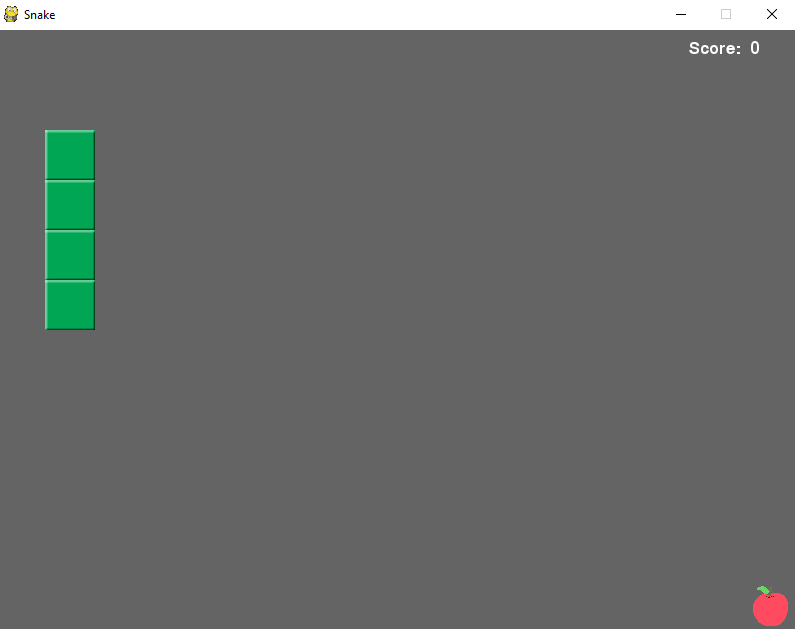
\includegraphics[scale=0.3]{snake}
	\caption{Our snake game UI}
	\label{fig:snake}
\end{figure}

\par The first thing we need for our agent was to implement a way to tell the agent the state of the game, our environment state. The way we structured our state is shown on the picture \ref{fig:snakeenv} below:

\begin{figure}[h]
	\centering
	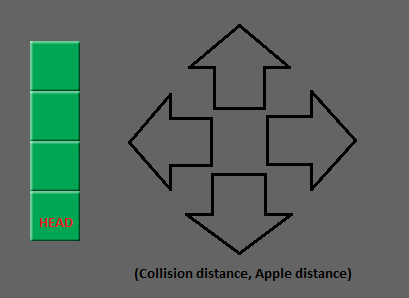
\includegraphics[scale=0.6]{snakeenv}
	\caption{Our snake game UI}
	\label{fig:snakeenv}
\end{figure}

\par As we can see we give the agent information in four directions. It is because the agent can only choose from four possible moves, top, down, left and right. The information is for every direction is the distance to the nearest collision and distance to the apple (the point). The distances were counted in multiple ways, because as it is obvious not all of them were equally good. The collision distances were almost always the same - how many moves in this direction snake needs to make to die, the apple distance though varied. We started from Euclidean distance to the apple from every 'next possible move' and finally based our model on a distance which gave zero when the apple was not in this direction at all and binary 0/1 when apple was in the direction given, with partial points in the range from 0 to 1 on apple being somewhere diagonally. So finally the state is counted in a given way presented with a simple algorithm \ref{state}:


\begin{algorithm}	
	\caption{Count state}\label{state}	
	\begin{algorithmic}[1]
		\Procedure{CountState}{}
		\State $\textit{applePos} \gets \text{position of the }\textit{apple}$
		\State $\textit{snakePos} \gets \text{position of }\textit{head}$
		\For{\texttt{d in directions}}
		\State $\textit{collisionD} \gets \text{distance to the nearest Wall/Snake in this direction}$
		\EndFor
		\For{\texttt{d in directions}}
		\If {$\textit{apple} \text{ is in}\textit{ d}$}
		\State $\text{add 1 to }\textit{state}$
		\EndIf
		\EndFor
		\If {$\textit{appleD} \text{ is }\textit{ empty}$}
		\State $\text{count partial } \textit{apple} \text{ distance }$
		\EndIf
		\Return $\textit{collisionD }\text{ + }\textit{apple}$
		\EndProcedure
	\end{algorithmic}
\end{algorithm}

\newpage

\par The only problem which we tried to solve and still didn't find the proper answer to is, if our state vector has only positive values (let us make this assumption), should the neural network be able to make out the subtle differences that some cells in the vector, if they are positive, give the model greater chance of getting a bigger reward, on the other hand some other positive values might stand for negative things - like collisions. Are the neural networks sophisticated enough to catch that? We would surely assume that it should but we did have some problems when we tried this method for collision checking.

\par This was presented the final way of counting the state before putting it into the neural network which is set to provide us with the values with which the neurons corresponding to each action/move is fired. From the neurons activity the agent is choosing the mostly rewarded action and that's how the process is going in an iterative way. 

\par The problem of giving the agent a proper reward is also important. As mentioned before reward is the key factor that is enabling the Agent in Q Learning to teach itself how to perform well (according to what we, humans, tell him is a good way of acting). To give the best outcomes reward is given as a real number from a range \begin{math} (0,1) \end{math}. Having normalised reward makes some problems more visible, cause the range is small enough for us to notice and count easily the reward percentage. 

\par We tried various rewards from binary to real and normalised and also not normalised at all. As it seems to be, normalised reward do gives the best outcome but sometimes, when it is too precise it gives a feeling of guiding the snake holding a carrot on the stick, instead of actually teaching him. But this is a subject of a rather different dispute. 

\par Our reward we agreed upon can be counted in a such way, presented below on \ref{reward}:

\begin{algorithm}	
	\caption{Count reward}\label{reward}	
	\begin{algorithmic}[1]
		\Procedure{CountReward}{}
		\If {$\textit{snake} \text{ is not}\textit{ alive}$}
		\Return $\textit{deathReward}$
		\Else
			\State $\textit{appleDist} \gets \text{distance from the }\textit{apple}$
			\If {$\textit{appleDist} \text{ is }\textit{0}$}
			\Return $\textit{eatReward}$
			\Else
			\Return $\textit{liveReward} \text{ + } \textit{eatReward / appleDist}$
			\EndIf
		\EndIf
		\EndProcedure
	\end{algorithmic}
\end{algorithm}

\par It is crucial to remember that we need to reward for getting the point, but staying alive is also a good feat. In a learning process when the game has more complex goals, reward must be somehow split between those things and we have to decide what is more valuable and how to balance the output given for the agent.

\par As we have learned it is very hard to train the agent the importance of both living and eating apples, thus getting points. Changing the reward from a lot points for living and less points for eating led to the Agent neglecting the point collecting whatsoever but focusing on getting to the point where the apple was is also hard because the Agent has to move around in the 'city metrics', having to chose only from four directions. The apple distance itself (counted as a percentage) is also not the best way for counting the reward because the distance which we can get changing our current position to some other is at least as much important as is the direction right. Also how to balance getting closer to the apple with getting closer to the wall and a spike of the negative values? 

\par Complicated environments must have it very hard to present the right reward for the right action, optimizing for gains and losses. 

\par On Game Over the environment is taken back to the starting state which is having the snake of length four, facing the bottom direction with an apple in a random spot of the board. The neural network is preserved with every iteration and the information is later used for training.

\subsection{Training}

\par Apart from iterative information collection, it is important to train the agent, based on its previous experiences. Our training at first was done every thousand game, but we figured out that the results were not too good, so the final training is done after every game. And it last the length of the game.

\par Training is based on a list of samples collected from the agent previous actions and given rewards. One record in a training list is a tuple: 

\begin{equation}
QRecord = (Previous State, Reward, Action, Next State, Game Over)
\end{equation}

\par The relation between the \textit{Previous State} and the \textit{Next State} is that between them the agent chose to perform \textit{Action}. \textit{Reward} is given to us by the environment and \textit{Game Over} component is telling us if after the \text{Action} the game has ended. In this sense \textit{Game Over} is an additional element helping the agent understand the environment and the rules of the game. 

\par Having the \textit{Game Over} information for a record we do not use the full formula, this is the Q equation to count the training output, because it involves predicting the next state, next state in case of game being over is None or a new game, so we just input the reward given by the network.

\par During every game information from every move is collected to the list of previous actions, and then the batch is chosen for training, being split into mini batches, so that every training session would be split into separate smaller trainings. Every smaller training is based on inputting the collected mini batch into the neural network. 

\par So our training is flexible in a sense that it can be done in many stages of the learning process. The training still does not break the no-teacher policy, because the agent is only tweaking the model based on previous experiences. It is important for a programmer to change the frequency and locations of the trainings because it can greatly affect the results. 

\newpage

\par Our training is working in a very simple way which is presented in a algorithm \ref{train} below:

\begin{algorithm}
	\caption{Train model}\label{train}
	\begin{algorithmic}
		\Procedure{Train model}{}
		\State  $\textit{n} \gets \text{(0, 10)}$
		\State $\textit{batchSize} \gets \text{random size in (0, len(} \textit{ExperienceList} \text{)}$	
		\State $\textit{miniBatchSize} \gets \text{batchSize/n}$
		\For{\texttt{miniBatch} \textbf{in} \texttt{batch}}
		\For{\texttt{elem} \textbf{in} \texttt{miniBatch}}
		\State $\text{add }\textit{elem.PreviousState} \text{ to } \textit{trainInput}$
		\If {$\textit{elem.GameOver == True}$}
		\State $\text{add }\textit{elem.Reward} \text{ to } \textit{trainOutput}$
		\Else
		\State $\text{add } \textit{(1 - gamma) * elem.Reward + gamma *} \newline \text{ model.predict(} \textit{elem.NextState} \text{) to } \textit{trainOutput}$
		\EndIf
		\EndFor
		\EndFor
		\State $\textit{model.train} \text{ with} \textit{train.Input, train.Output}$
		\EndProcedure
	\end{algorithmic}
\end{algorithm}
 
\par As we have learned there are numerous training practises and the variation of this one if so far the most common we have encountered. In any case of data-overflow we have easy mechanisms to cut the great explosion of filling up the memory with cutting the maximal length of the Q records list. This is a good safety mechanism, we need to remember that data collected later on is usually way more valuable than data collected on the beginning, when the model is not trained almost at all.

\par Having that in mind we have also created a way to input and output our model into a \textit{.csv} file. Thanks to this practise we can train our model partially, save data to file, and keep training it later on. Also we can compare models trained with different approaches, with various ways of counting the state (distance to the apple) and various training methods. 

\par As a good practice in Machine Learning we also put something called \textit{Epsilon} which is a percentage with which random moves are chosen instead of predicting rewards from our neural network. This enables the model to explore new paths, and prevents from falling into a local maximum. As the model is getting better in predicting the correct moves, the \textit{Epsilon} is decreasing, in our case we decrease it by every thousand games.

\section{Results}

\subsection{Neural network}

\par Choosing the neural network over a basic Q table was an interesting choice for a couple of reasons. Such networks enable us to work with it with a very low input in building the model itself. Neural network is a sort of a standalone model that only needs the programmer to input the variable vector - information from the environment and also train the model when needed. Apart from that all the calculations and neuron activity is happening inside the network, we do not interact with that.

\par One of the problems we had is just that - the sole fact that the network is a very standalone entity and we cannot do much about what is happening inside of it once we input the vector of values. We were tweaking and changing both the reward system, and the distances (impulses getting to the Agent from the environment of the game) - what we called previously a state but the results were always almost accidental. After around 30.000 iterations, whatever the gamma or if there was a third layer in the network at all, the Agent was able not to die, but we could not teach him to pick the apples. And the only action that we could undertake is longer training and trying to expose the agent to such situations in which he failed to do what we wanted him to do. 

\par The hermetic structure of a neural network was sometimes hard to work with cause we were only left with working with just the values vector, leaving all the 'inside job' to the closed model of the network.

\subsection{Performance overall}

\end{document}
